\section{Problem resolution}
\label{sec:problem-resolution}
The first we have done in this project was testing that our program will actually work. As our first coding task we implemented the problem formulation that we described in the section \ref{sec:intro}, the problem reported has only the minimization function and it ensures that each node has only one edge incoming and only one edge outcoming. In this first part of this report, we will consider only the symmetric TSP so the resulting graph will be undirected. Until otherwise specified the following methods are testes with the file \href{http://comopt.ifi.uni-heidelberg.de/software/TSPLIB95/tsp/}{att48.tsp.}

\begin{figure}[h]
	\centering
	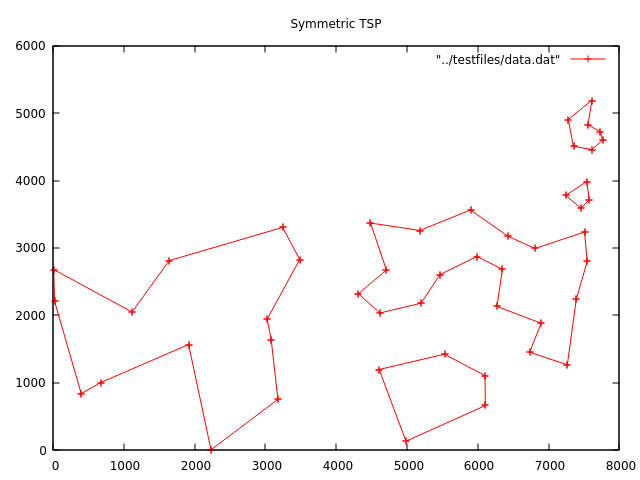
\includegraphics[width=0.6\textwidth]{images/symmetric_with_tours}
	\caption{The image represent att48.tsp solved with the problem formulation showed in section \ref{sec:intro}}
\end{figure}

As we can see the solution that CPLEX found doesn't contain a single tour but a lot of sub-tours. The TSP problem requires that all the nodes must be connected with only one cycle, to do that we implemented different solutions that we will see in this report, the following subsection will explore the basic formulation of the loop method (also known as benders) and some compact models (MTZ and GG).\\
Before the introduction of this methods we need to introduce the most known formulation to the loops problem inside the TSP. Dantzig, Fulkerson and Johnson \cite{dantzig} introduced what it can be said to be one of the most efficient approach:

\begin{equation}
	\sum_{i\in S}\sum_{j \in S}x_{ij}\le |S|-1; \quad \forall S \subset\{2, \dots, n\}, \; |S|\ge 2
\end{equation}

Where $S$ is the set of nodes that are in the solution. This equation implies that the number of edges in the solution cannot be greater that $|S|-1$.

The main problem with this formula is that it produces a great number of constraint ($O(2^n)$) and it makes it unfeasable even for relatevely small amount of nodes.

\subsection{Loop model}
\label{sec:loop}
This method is easier to implement and also easier to understand. This process that we are going to describe is also known as benders decomposition and it is based on the principle of the divide-and-conquer.

%%TODO riscrivere meglio vala'
The basic algorithm is the following: we give CPLEX the same model as before but this time we check if the solution has some sub-tour, if yes then we apply the loop method to each cycle found. Essentially it creates a new constraint and adds it to the problem, the constraint that is going to block the formation of the cycles in the next call of CPLEX. \\
Let's make an example, we have a cycle that is composed by five nodes and consequently by five edges that forms the sub-tour; the constraint we build forces the software to connect those five edges with a maximum of four (number of nodes - $1$) edges, this method must be applied to all the sub-tours found in the solution, then we call again CPLEX to solve the problem. If the problem has again some cycles inside we will apply again the loop method until the nodes are connected with only one cycle.

\begin{figure}[h]
	\centering
	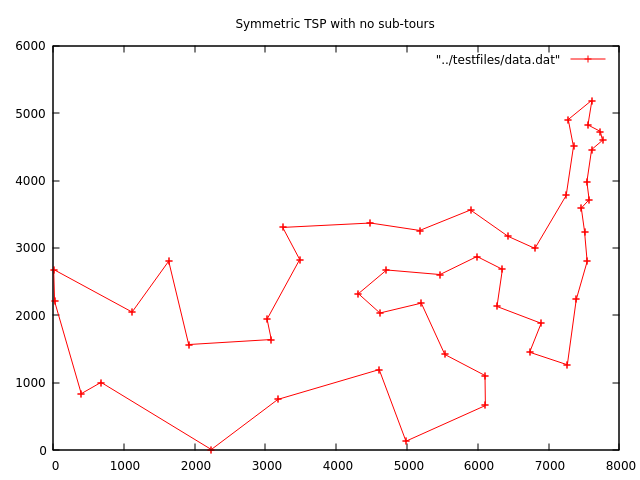
\includegraphics[width=0.6\textwidth]{images/symmetric_with_no_tours}
	\caption{The image represent att48.tsp solved with the loop method described in section \ref{sec:loop}}
\end{figure}

As we can see this time the solution found have no sub-tours and in particular this one was found in circa $0.3$ seconds with a total of 7 iterations where there were added 22 constraints in order to obtain this final solution.

\subsubsection{Particularity of the variable creation in the symmetric TSP}
In the setup section (\ref{cap:2_int}) we have seen how the variable and constraints are implemented inside cplex, we have also seen how we can refer to a variable when using the callable library, by simply using its "position" inside the variable array. It is immediately noticeable that the order in which we create them is really important and allow us to know exactly the position of each variable inside that array.

The way we managed the variables is the following: we think them as they were inside a matrix where the rows are the starting node and the columns are the arriving node. We can see an example in the figure \ref{img:full_matrix}.

\begin{figure}[h]
	\centering
	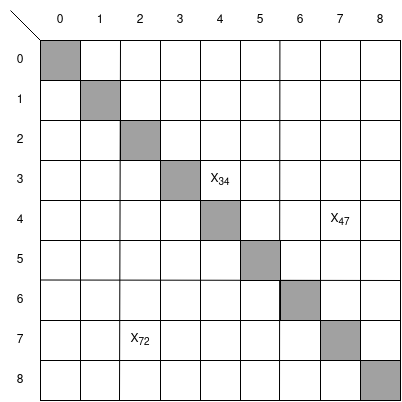
\includegraphics[width=0.55\textwidth]{images/full_matrix}
	\caption{The image represent the matrix method we used to reference the variable inside CPLEX}
	\label{img:full_matrix}
\end{figure}

In this way the is it really simple to find the number of the variable we want to reference, for example if we want to use the index of $x_{34}$ we just need to compute this $3 * (\text{number of nodes}) + 4$ and thats it.

In the particular case of the simmetric TSP the path from $i$ to $j$ and $j$ to $i$ is the same so we don't need all the matrix that we have just showed. So in order to easily obtain the number we image a matrix as the one in the figure \ref{img:full_matrix_simm}, this time all the cells that are in gray are not used since the useful values are saved in the other cells since $x_{ij}$ have the same value than $x_{ji}$.


\begin{figure}[h]
	\centering
	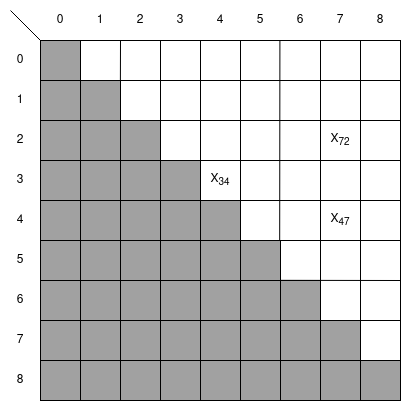
\includegraphics[width=0.55\textwidth]{images/full_matrix_simmetric}
	\caption{The image represent the matrix method we used to reference the variable inside CPLEX in the case of the simmetric TSP. In this case half of the matrix is not used since the values that were in the gray cells are the same of its "corrisponding white cell" since $x_{ij}$ have the same value than $x_{ji}$. In fact the value $x_{72}$ in the figure \ref{img:full_matrix} is transposed into $x_{27}$.}
	\label{img:full_matrix_simm}
\end{figure}

\subsection{Miller-Ticker-Zemlin model}
\label{sec:mtz}
As said in section \ref{sec:problem-resolution} the Miller-Ticker-Zemlin model is a compact model for the resolution of the TSP problem but, instead of the symmetric problem we have faced so far, it can be applied only to the asymmetric one. In fact in this case we will consider $x_{ij}$ and $x_{ji}$ two completely different paths with different lenghts (in our particular case the two path will have the same lenght). This model can delete all the sub-tours in a given problem: the current formulation of the constraints need the construction of an additional variable $u_i$ which is used to denote the position of node $i$ in the tour, here it is its formulation as described in (CITATION):

\begin{equation}
\label{eqn:big-m}
	u_i-u_j+nx_{ij}\le n-1; \quad i,j\in \{2, \dots, n\}, i \not= j
\end{equation}
\begin{equation}
	\label{eqn:u-bound}
	u_i \in \Re; \: i \in V:i>1
\end{equation}

Where $V$ is the set of nodes. In the original paper the variables $u_i$ were unrestricted but they can be restricted without compromising the solution of the asymmetric TSP, so we can rewrite \ref{eqn:u-bound} as:

\begin{equation}
	u_1=1
\end{equation}
\begin{equation}
	2\le u_i \le n; \: i\in V:\:i>1
\end{equation}

This formulation compared with \cite{dantzig} has a better complexity since the number of constraints used are $O(n^2)$ that is a lot better compered to $O(2^n)$ of the previous model.

\subsubsection{Implementation of the model}
Essentially the model implies that the nodes in the tour must be numbered in increasing order, from number $1$, that is the start node, to $n$. In fact the formula \ref{eqn:big-m} is simply a Big-M constraint that force the node $j$ to have an $u$ greater than node $j$ if the arc $x_{ij}$ is selected. Now that we explained what the \ref{eqn:big-m} means we can rewrite it as a Big-M constraint in order to see the reference better:

\begin{equation}
	u_j\ge u_i+1-M(1-x_{ij})
\end{equation}

And than setting $M$ to $n$ and doing some basic algebra we can see the relation between them.

Now that we have explained the formula we can start explaining the three implementation of the the MTZ model:

\begin{itemize}
	\item standard constraints: in this case all the constraints wrote in \ref{eqn:big-m} are directely saved into the problem and than the problem is solved by CPLEX;
	\item lazy constraints: here the constraints are not always applied to the problem, as the name can suggest they are applied lazily, so CPLEX use them only when necessary or not before needed;
	\item indicator constraints: in the first two cases the Big-M trick is used to trigger a constraint when a particular variable assumes a predermined value, but this method (Big-M) is not always preferable since can behave in unstable ways. Thats why a good implementation of \ref{eqn:big-m} is the usage of the indicator constraints: CPLEx automatically activate the constraint $u_j\le u_i-1$ when the $x_ij$ assume the user passed value.
\end{itemize}


\subsection{Gavish and Gaves model}
The second compact model we have implemented in our project is the one proposed by Gavish and Gaves (this model will be called from now on GG) and it is based on the single commodity flow: the arcs in fact will be considered as pipes. As the MTZ model also this one can only be applied to asymmetric problem instead of the symmetric one.\\
Based on [Put here gavish and gaves model] the additional constraints to put in the model are the following:

\begin{equation}
	\label{eqn:linking}
	y_{ij}\le (n-1)x_{ij}
\end{equation}

\begin{equation}
	\label{eqn:flow_first}
	\sum_{j;j\not=1}y_{1j}=n-1
\end{equation}

\begin{equation}
	\label{eqn:flows}
	\sum_{i;i\not=j}y_{ij}-\sum_{k;i\not=k}y_{jk}=1
\end{equation}

Where the variable $y_{ij}$ is a variable created to represent the flow of the arc. The equations \ref{eqn:flow_first} and \ref{eqn:flows} say that from the first node starts a flow of $n-1$ and than for each node of the path find the flow needs to lower its value by 1. The first constraint we introduced (\ref{eqn:linking}) is the one that allows the flow to take place only if the arc is selected.

As in section \ref{sec:mtz} we used the Big-M method to create the constraint \ref{eqn:linking}, so its implementation is the same as before.

\subsection{Performance Analysis}